
\newpage
\section{Conclusion}
\par A simplified numerical model of the sensors was developed and integrated into the Simulink environment to evaluate the system behavior under realistic feedback conditions. This model accounts for the fundamental dynamics of the sensing elements, ensuring that the simulated control signals closely approximate the behavior of the physical hardware.

\par The final simulation results are presented below. The data demonstrates the efficacy of the control architecture when subjected to the modeled sensor characteristics.

\begin{figure}[H]
    \centering
    
\includegraphics[width=0.4\linewidth]{Body/Images/final_sensors.pdf}
    \caption{Controlled system feedback}
    \label{fig:no_compensator}
\end{figure}

\par Following the simulation phase, the system was validated through experimental testing. The experimental results, illustrated in the subsequent figures, show a high degree of correlation with the numerical predictions. Notably, the steady-state performance remained within highly acceptable tolerances, with the angular error for $\beta$ oscillating within $\pm0.5^\circ$ and the error for $\alpha$ maintained between $\pm1^\circ$.

\begin{figure}[H]
    \centering
    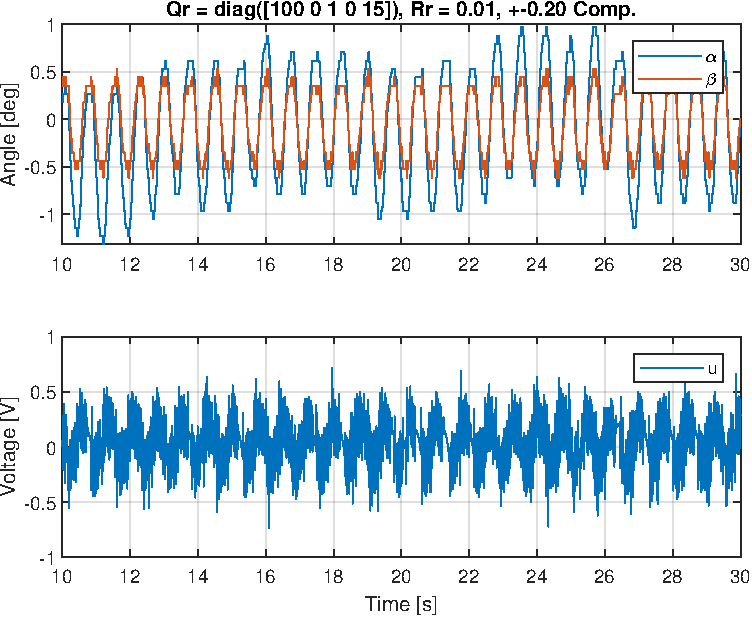
\includegraphics[width=0.4\linewidth]{Body/Images/1teste.pdf}
    \caption{Controlled system feedback}
    \label{fig:no_compensator}
\end{figure}

\par These results indicate that the control system effectively compensates for the inherent non-linearities of the plant. The narrow oscillation ranges in both $\alpha$ and $\beta$ confirm that the integrated deadzone compensator and sensor models provide sufficient precision for the requirements of the application, achieving a stable and robust response in the physical implementation.